%!TEX root = TableSummarizationDemo.tex

\section{Demo Overview} \label{sec:demo} 
In our demo, we will show our prototype implementation of a system equipped with smart drill-down. The implementation includes a web interface. We have included two datasets, a marketing survey, and the US Census, which users can explore using smart drill-down. Figure~\ref{fig:interface} shows a screenshot of the web interface. 

At the top, users can set the number of new rules to display in response to every smart drill-down. The second setting is a parameter called max weight, which trades off the accuracy of the displayed rule list for processing time. Briefly, our system only considers displaying rules that have weight $\leq$ the max weight. As long as the weight of all rules in the optimal rule-list is less than this parameter, our system displays the optimal rule-list. We observe that a value of around $5$ works well for the Size weighting function. Weighting functions with higher weight values need a higher value for this parameter. 

The third parameter the can set if the weighting function. In general, our approximation algorithm works for any monotonic weighting function. But for ease of use of the web interface, we have hardcoded a few different weighting functions, that can be selected using the drop-down list in the interface. Below, the interface displays the set of columns of the database table being explored. Each column has three options: `Default', `Ignore', and `Force'. Choosing the Ignore option causes the column to be ignored, (so the weight given to a rule with a value in that column is set to that of a rule with a $\star$ value in that column). Choosing the Force option forces every displayed rule to have a non-$\star$ value in that column. 

Finally, the actual interactive table summary is displayed below. The plus and minus buttons before the rules can be used to drill-down and reverse previous drill-downs. For instance, in the figure, the user has performed a single drill down using the Size weighting function (which sets weight to the number of non-star values of a rule), and choosing the Force option for the Occupation column, and Ignore for Gender and Time in Bay Area columns. As a result, the displayed rule-list (the three rules below the first one) all have a non-$\star$ value in the Occupation column, and only $\star$ values in the Gender and Time in Bay Area columns. Unlike in a traditional drill-down, the displayed rules also have non-$\star$ values in columns other than Occupation. 

\begin{figure*}[ht]
\vspace{-5pt}
\centering
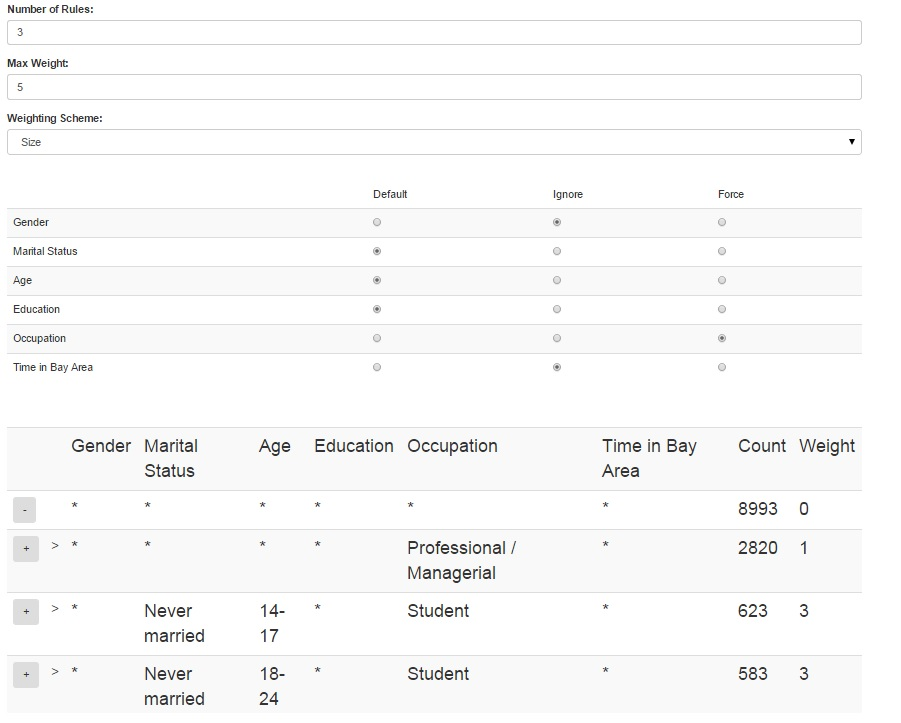
\includegraphics[width=160mm,frame]{graphs/tsapp_screenshot.jpg}
\vspace{-10pt}
\caption{The web interface of our system \label{fig:interface}}
\vspace{-20pt}
\end{figure*}